\chapter{Tecnologie utilizzate}
In questo capitolo verranno descritte le attività preliminari per la realizzazione di questo progetto, le tecnologie utilizzate
unitamente alle motivazioni legate all'uso di questi sistemi rispetto ad altri. In particolare nel capitolo successivo verranno 
approfonditi a livello pratico i sitemi di raccomandazione Memory-based i quali sono stati utilizzati per l'implementazione della
soluzione. 

%% AGGIUNGERE RIFERIMENTI AI CAPITOLI SUCCESSIVI E INDICARE QUALI SONO LE PARTI CHE POI SONO STATE IMPLEMENTATE NELLA 
%% SOLUZIONE DI QUESTO PROGETTO

\section{Perché Python e Django}
\paragraph{Python}
Python è un linguaggio di programmazione ad alto livello, orientato agli oggetti, adatto, tra gli altri usi, a sviluppare applicazioni 
distribuite, scripting, computazione numerica e system testing; ideato e rilasciato pubblicamente per la prima volta nel 1991 dal suo 
creatore Guido van Rossum, programmatore olandese.

Python supporta diversi paradigmi di programmazione, come quello object-oriented (con supporto all'ereditarietà multipla), quello 
imperativo e quello funzionale, ed offre una tipizzazione dinamica forte. È fornito di una libreria built-in estremamente ricca, che 
unitamente alla gestione automatica della memoria e a robusti costrutti per la gestione delle eccezioni fa di Python uno dei linguaggi 
più ricchi e comodi da usare.

Inoltre è anche semplice da usare e imparare. Python, nelle intenzioni di Guido van Rossum, è nato per essere un linguaggio 
immediatamente intuibile. La sua sintassi è pulita e snella così come i suoi costrutti, decisamente chiari e non ambigui. I blocchi 
logici vengono costruiti semplicemente allineando le righe allo stesso modo, incrementando la leggibilità e l'uniformità del codice 
anche se vi lavorano diversi autori.

Un aspetto inusuale del Python è il metodo che usa per delimitare i blocchi di programma, che lo rende unico fra i linguaggi più diffusi.

\lstset{style=python_code_style}
\begin{lstlisting}[language=Python, caption={Esempio di programma in Python}]
# Testing if two strings are equals
def test(got, expected):
	if got == expected:
		prefix = ' OK '
	else:
		prefix = ' X '
	print('%s got: %s expected: %s' % (prefix, repr(got), repr(expected)))

def main():
	print('verbing')
	test('hail', 'hailing')
	test('swiming', 'swimingly')
	test('do', 'do')

if __name__ == '__main__':
	main()
\end{lstlisting}

Nei linguaggi derivati dall'ALGOL come Pascal, C e Perl, i blocchi di codice sono indicati con le parentesi oppure con parole chiave 
(il C ed il Perl usano { }; il Pascal usa begin ed end). In questi linguaggi è solo una convenzione degli sviluppatori il fatto di 
indentare il codice interno ad un blocco, per metterlo in evidenza rispetto al codice circostante. In Python invece di usare parentesi 
o parole chiave, usa l'indentazione stessa per indicare i blocchi nidificati in congiunzione col carattere "due punti" (:). Si può usare 
sia una tabulazione, sia un numero arbitrario di spazi, ma lo standard Python è di 4 spazi. 

Python è un linguaggio pseudocompilato: un interprete si occupa di analizzare il codice sorgente (semplici file testuali con 
estensione .py) e, se sintatticamente corretto, di eseguirlo e non esiste una fase di compilazione separata (come 
avviene in C, per esempio) che generi un file eseguibile partendo dal sorgente. \cite{python-documentation}

\paragraph{Django}
Django è un web framework di alto livello basato su Pyhton che permette di sviluppare rapitamente e con tutti i presupposti per un sistema sicuro, un sito web
perfettamente mantenibile, Django si occupa della maggiori grane del sviluppo web, così da permetterti di concentrarti sulla scrittura della tua app; inoltre 
è open-source e ha una comunità attiva, una documentazione completa e sempice da consultare.

Django aiuta a scrivere software con le seguenti caratteristiche \cite{django-documentation}:
\begin{description}
	\item[Versatile]: è usato per la creazione di praticamente tutti i tipi di siti web, a partire a sistemi per la gestioni di contenuti e wiki,
	social network e siti di notizie; può lavorare con qualunque client-side framework, gestire contenuti in quasi tutti i formati (inclusi HTML, 
	RSS feeds, JSON, XML, etc). Internamente permette la scelta e l'implementazione di qualsiasi funzionalità (es. molti dei database più popolari, etc.).
	\item[Sicuro]: aiuta gli sviluppatori a evitare gli errori più comuni in merito alla sicurezza provvedendo un framework costruito per eseguire 
	le operazioni in modo corretto e sicuro. Ad esempio, Django fornisce un modo sicuro per gestire gli account degli utenti e le relative
	password, evitando errori comuni come inserire informazioni riguardanti la sessione dell'utente nei cookies dove sarebbero vulnerabili (invece i cookie
	contengono soltanto una chiave, e i valori effettivi sono salvati nel database) o salvare direttamente una password invece di una hash password.
	\item[Mantenibile]: il codice di Django è scritto seguedo i principi e i pattern che incoraggiano la creazione di codice mantenibile e riusabile. Inoltre
	particolare, fa uso del principio "Don't Repeat Yourself" (DRY) così da ridurre al minimo le duplicazioni non necessarie, diminuendo la quantità di codice.
	Django raggruppa parti di codice legto in moduli seguendo le linee guida del pattern Model View Controller (MVC).
	\item[Portatile]: Django essendo scritto in Python, un linguaggio multi piattaforma, lo rende indipendente dal sistema operativo eseguito sul server, che
	sia Linux, Windows o Mac OS X. Per di più, Django è ben supportato da molti web hosting provider, che spesso provvedono a specifche infrastructure e 
	e documentazione per l'hosting di siti web in Django.
\end{description}


Un tradizionale sito web attende delle richieste HTTP dal browser web (o altri client). Quando viene ricevuta una richiesta, di tipo POST o GET, l'applicazione 
legge le informazioni contenute nel URL e altri possibili dati a seconda del tipo di richiesta. A seconda della richiesta è possibile che vengano letti o 
scritti dati da un database o altre operazioni che portino al soddisfacimento della richiesta. A quel punto l'applicazione ritorna una risposta al browser 
web, spesso in modo dinamico, creando una pagina HTML da mostrare in cui è possibile inserire o recuperare dati in placeholder in un template HTML.

\newpage

\begin{figure}[ht!]
    \centering
	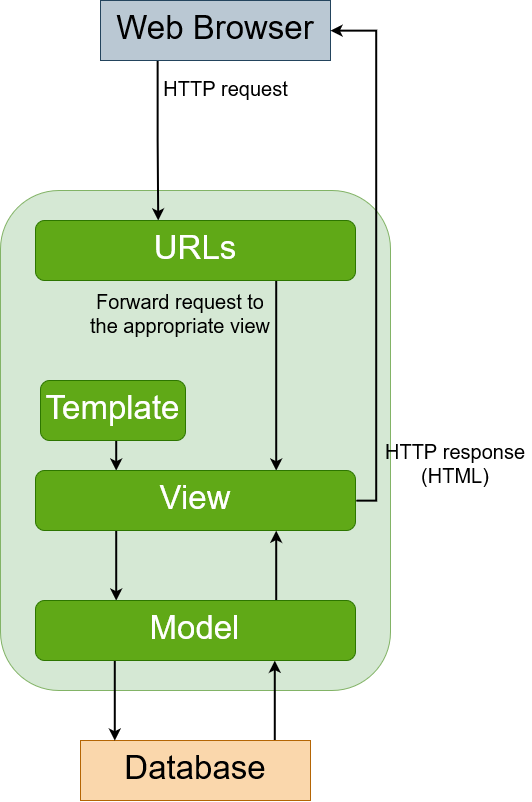
\includegraphics[scale=0.3]{images/Django_doc.png}
	\caption{Schema generico di funzionamento di un applicativo web sviluppato con Django}
	\label{fig:django_doc}
\end{figure}

Un'applicazione web in Django tipicamente raggruppa il codice che gestisce questi diversi passaggi in file separati \cite{mdn-django-documentation}:
\begin{description}
	\item[URL]: mentre è possibile processare richieste da qualsiasi URL attraverso unas singola funzione, è più mantenibile scrivere diverse funzioni chiamate
	View per gestire ogni risorsa. un URL mapper è usato per reindirizzare le richieste HTTP alla view corretta in base all'URL della richiesta; inoltre è 
	possibile controllare se nell'URL è presente un particolare pattern di stringhe o numeri, e passare di conseguenza la richiesta alla funzione appropriata
	come dati da elaborare.
	\item[View]: una View è una funzione che gestisce le richieste HTTP, e restituisce una risposta HTTP. Le view accedono ai dati necessari per soddisfare la 
	richiesta attraverso i Model, e delegano la formattazione delle risposte ai template. 
	\item[Model]: i Model sono oggetti in Python che definiscono la struttura dei dati dell'applicazione, e provvedono meccanisci per gestirla (add, modify, 
	delete) e query per interpellare il database.
	\item[Template]: un template è un file di testo che definisce la struttura o il layout di un file (come una pagina HTML), attraverso placeholder per 
	rappresentare il contenuto effettivo. Una View può creare dinamicamente una pagina HTML usando un template HTML, popolandolo con dati presi dal Model. 
\end{description}

\section{Docker}
Docker è una piattaforma software che permette di creare, testare e distribuire applicazioni con la massima rapidità. Docker raccoglie 
il software in unità standardizzate chiamate \textit{container} che offrono tutto il necessario per la loro corretta esecuzione, incluse librerie, 
strumenti di sistema, codice e runtime. Con Docker, è possibile distribuire e ricalibrare le risorse per un'applicazione in qualsiasi ambiente, 
tenendo sempre sotto controllo il codice eseguito.

La tecnologia Docker utilizza solitamente il kernel di Linux e le sue funzionalità, come Cgroups e namespace, per isolare i processi in modo da poterli 
eseguire in maniera indipendente. Questa indipendenza è l'obiettivo dei container: la capacità di eseguire più processi e applicazioni in 
modo separato per sfruttare al meglio l'infrastruttura esistente pur conservando il livello di sicurezza che sarebbe garantito dalla 
presenza di sistemi separati.

\begin{figure}[ht!]
	\centering
	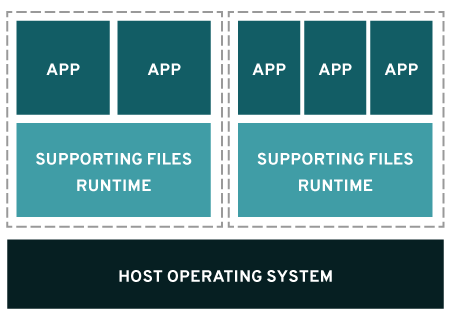
\includegraphics[scale=0.7]{images/Docker_Config_Container.png}
	\caption{Schematizzazione del contenuto di un Container in Docker}
	\label{fig:DCC}
\end{figure}

Gli strumenti per la creazione di container, come Docker, consentono il deployment a partire da un'\textit{immagine}, ciò semplifica la condivisione di 
un'applicazione o di un insieme di servizi, con tutte le loro dipendenze, nei vari ambienti.
Docker, considera i container come macchine virtuali modulari estremamente leggere, offrendo la flessibilità di creare, distribuire, 
copiare e spostare i container da un ambiente all'altro, ottimizzando così le app per il cloud.

I contenitori forniscono una modalità standard per impacchettare il codice della tua applicazione, le configurazioni e le dipendenze, in un oggetto singolo e 
condividono un sistema operativo installato sul server, operando come processi con risorse isolate, assicurando velocità, affidabilità e distribuzioni coerenti, 
indipendentemente dall’ambiente.

\section{Strutture dati gerarchiche}
Le tabelle di un database relazionale non sono gerarchiche (come nel XML), ma sono delle semplici liste piatte. I dati gerarchici sono 
constituiti da relazioni padre-figlio che non possono essere rappresentate in modo naturale nelle tabelle di questo tipo.
In questo caso, i dati gerarchici sono una collezione di informazioni dove ogni item ha un solo padre e nessuno o più figli
(ad eccezione del nodo radice che non ha un nodo padre); questo genere di rappresentazione delle informazioni, simili a un albero, 
può essere trovato in diversi ambiti di applicazione di un database, incluse discussioni su forum e mailing list, grafici di 
organizzazione di un business, categorie per gestire contenuti e categorie di prodotti. \\

\begin{figure}[ht!]
	\centering
	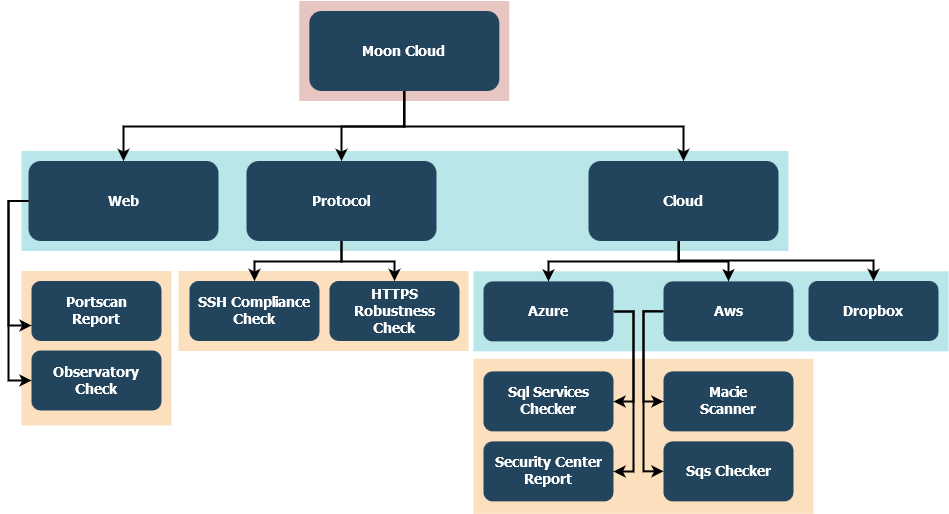
\includegraphics[scale=0.49]{images/MC_Rec_Tree.png}
	\caption{Esempio della rappresentazione gerarchica parziale dei dati nel progetto in questione}
	\label{fig:MC_Rec_Tree}
\end{figure}

%\newpage

Ci sono differenti modelli per poter gestire dati in modo gerarchico, i più importanti  presi in considerazione sono i seguenti:

\subsection{The Adjacency List Model}
Il primo approccio, e quello di più semplice implementazione, qui descritto è chiamato \textit{Adjacency List Model} o metodo ricorsivo;
è definito tale perchè il suo funzionamento si basa su una funzione che itera per tutto l'albero.\\
In questo modello, ogni item (nodo dell'albero) nella tablla contiene un puntatore al suo item padre; invece il nodo radice avrà un 
puntatore a un valore NULL per l'item padre.

La Tabella \ref{table:adjacency_list_model_table} è un esempio di possibile rappresentazione parziale dei dati nel database implementato 
in questo progetto secondo questo approccio, seguendo come riferimento la Figura \ref{fig:MC_Rec_Tree}.
 
\begin{table}[ht!]
\centering
\begin{tabular}[c]{| c | l | c |} 
	\hline
	id & name & parent \\ [0.5ex] 
	\hline
	\rowcolor{rootnodecell} 1 & Moon Cloud & NULL \\ [0.5ex] 
	\rowcolor{categorycell} 2 & Web & 1 \\ [0.5ex] 
	\rowcolor{categorycell} 3 & Protocol & 1 \\ [0.5ex] 
	\rowcolor{categorycell} 4 & Cloud & 1 \\ [0.5ex] 
	\rowcolor{evaluationcell} 5 & Portscan Report & 2 \\ [0.5ex] 
	\rowcolor{evaluationcell} 6 & Observatory Check & 2 \\ [0.5ex] 
	\rowcolor{evaluationcell} 7 & SSH Compliance Check & 3 \\ [0.5ex] 
	\rowcolor{evaluationcell} 8 & HTTPS Robustness Check & 3 \\ [0.5ex] 
	\rowcolor{categorycell} 9 & Azure & 4 \\ [0.5ex] 
	\rowcolor{categorycell} 10 & Aws & 4 \\ [0.5ex] 
	\rowcolor{categorycell} 11 & Dropbox & 4 \\ [0.5ex] 
	\rowcolor{evaluationcell} 12 & Sql Services Checker & 9 \\ [0.5ex] 
	\rowcolor{evaluationcell} 13 & Security Center Report & 9 \\ [0.5ex] 
	\rowcolor{evaluationcell} 14 & Macie Scanner & 10 \\ [0.5ex] 
	\rowcolor{evaluationcell} 15 & Sqs Checker & 10 \\ [0.5ex]
	\hline
\end{tabular}
\caption{Esempio di una possibile tabella per gestire dati in modo gerarchico secondo l'Adjacency List Model}
\label{table:adjacency_list_model_table}
\end{table}

Il vantaggio di usare questo modello sta nella sua semplicità di costruzione, sopratutto a livello di codice client-side, 
e di restituzione dei figli di un nodo. Mentre diventa problematico se si lavora in puro codice SQL e nella maggior parte dei linguaggi 
di programmazione, è lento e poco efficente, perchè è necessaria una query per ogni nodo dell'albero, e visto che ogni query impiega 
un certo periodo di tempo, questo rende la funzione molto lente quando si lavora con alberi di grandi dimensioni, inoltre molti linguaggi 
non sono ottimizzati per funzioni ricorsive. Per ogni nodo, la funzione crea una nuova istanza di se stessa e ogni istanza occupa 
una porzione di memoria e impiega un certo tempo per inizializzarsi, più grande è l'albero e più questo processo sarà portato a termine 
in maggior tempo.

\subsection{The Nested Set Model}
Il secondo approccio analizzato è il \textit{Nested Set Model}, che permette di osservare la gerarchia in un modo diverso, non 
come nodi e linee (come se fosse un albero), ma come container innestati. \\

\begin{figure}[ht!]
	\includegraphics[scale=0.30]{images/MC_Rec_NSM_Container.png}
	\caption{Esempio della gestione di dati in modo gerarchico secondo il Nested Set Model, utilizzando dati presi dal database del 
	progetto in questione}
	\label{fig:MC_Rec_NSM_Container}
\end{figure}

Con questo sistema la gerarchia viene mantenuta, secondo il principio cui un nodo padre contiene e suoi figli e questa forma di 
gerarchia viene mantenuta in tabella attraverso l'uso di due attributi aggiuntivi come è possibile osservare dalla Tabella 
\ref{table:nested_set_model_table} seguente. 

\begin{table}[ht!]
\centering
\begin{tabular}[c]{| c | l | c | c |} 
	\hline
	id & name & lft & rght \\ [0.5ex] 
	\hline
	\rowcolor{rootnodecell} 1 & Moon Cloud & 1 & 100 \\ [0.5ex] 
	\rowcolor{categorycell} 2 & Web & 86 & 99 \\ [0.5ex] 
	\rowcolor{categorycell} 3 & Protocol & 80 & 85 \\ [0.5ex] 
	\rowcolor{categorycell} 4 & Cloud & 4 & 29 \\ [0.5ex] 
	\rowcolor{evaluationcell} 5 & Portscan Report & 91 & 92 \\ [0.5ex] 
	\rowcolor{evaluationcell} 6 & Observatory Check & 89 & 90 \\ [0.5ex] 
	\rowcolor{evaluationcell} 7 & SSH Compliance Check & 83 & 84 \\ [0.5ex] 
	\rowcolor{evaluationcell} 8 & HTTPS Robustness Check & 81 & 82 \\ [0.5ex] 
	\rowcolor{categorycell} 9 & Azure & 13 & 26 \\ [0.5ex] 
	\rowcolor{categorycell} 10 & Aws & 5 & 12 \\ [0.5ex] 
	\rowcolor{categorycell} 11 & Dropbox & 27 & 28 \\ [0.5ex] 
	\rowcolor{evaluationcell} 12 & Sql Services Checker & 22 & 23 \\ [0.5ex] 
	\rowcolor{evaluationcell} 13 & Security Center Report & 20 & 21 \\ [0.5ex] 
	\rowcolor{evaluationcell} 14 & Macie Scanner & 8 & 9 \\ [0.5ex] 
	\rowcolor{evaluationcell} 15 & Sqs Checker & 10 & 11 \\ [0.5ex]
	\hline
\end{tabular}
\caption{Esempio di una tabella per gestire dati in modo gerarchico secondo il Nested Set Model}
\label{table:nested_set_model_table}
\end{table}

Come è possibile osservare dalla Tabella \ref{table:nested_set_model_table} la gerarchia dei dati viene rappresentata attraverso l'uso 
degli attributi 'left' e 'right' per rappresentare l'annidamento dei nodi (il nome delle colonne: 'left' e 'right', hanno significati 
speciali in SQL; per questo motivo si identificano questi campi con i nomi 'lft' e 'rght'). \\

\begin{figure}[ht!]
	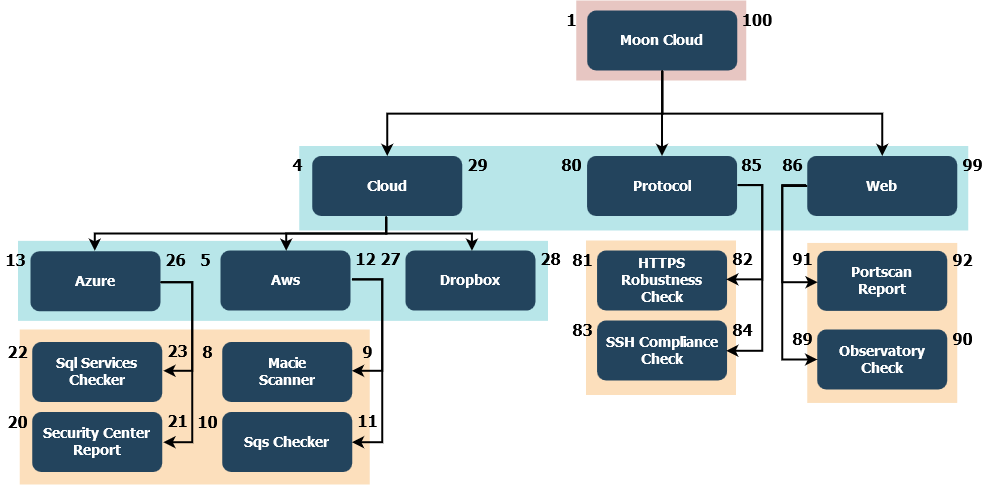
\includegraphics[scale=0.40]{images/MC_Rec_NSM_Tree.png}
	\caption{Esempio della gestione di dati in modo gerarchico secondo il Nested Set Model, utilizzando dati presi dal database del 
	progetto in questione}
	\label{fig:MC_Rec_NSM_Tree}
\end{figure}

L'assegnazione di questi valori ad ogni nodo viene effetuata seguendo questo procedimento: ogni nodo dell'albero viene visitato due volte, 
assegnando i valori in ordine di visita, e in entrambe le visite. Quindi vengono associati ad ogni nodo due numeri, memorizzati come 
due attributi. 
Più precisamente si inizia la visita dell'albero partendo da sinistra e continuando verso destra, un livello alla volta, scendendo per ogni
nodo i suoi figli, assegnando i valori al campo left, prima di assegnare un valore al campo right, e successivamente si continua verso 
destra. Questo approccio è chiamato \textit{Modified preorder tree traversal algorithm} (MPTT). A partire da questa tecnica è stato 
ideata la struttura della tassonomia delle evaluation e dei controlli implementate nella soluzione proposta in questa tesi, con 
l'ausilio di un package di Python chiamato MPTT.

Più semplicemente se si osserva la parte superiore della Figura \ref{fig:MC_Rec_NSM_Container} possiamo notare che la numerazione dei nodi, viene
effettuata a partire da container più esterno da sinistra e continua verso destra.

A prima vista questo approccio può sembrare più complicato da comprendere rispetto all'Adjacency List Model, ma quest'utlimo è
molto più veloce quando si vuole recuperare i nodi, visto che basta una query, mentre è più lento per operazioni di aggiornamento e 
cancellazione dei nodi; in quest ultimo il grado di complicatezza dell'operazione è determinato dal nodo che si vuole cancellare, a 
partire dal caso più semplice, il nodo foglia (un nodo senza figli) fino al caso più complicato, quando si vuole cancellare il nodo 
radice.

\newpage

\section{Sistemi di raccomandazione}
Un sistema di raccomandazione (\textit{Recommendation System}) è un sistema che consiglia ad utenti uno o più item esistenti 
in un database. L'\textit{item} è un qualsiasi cosa di interesse agli utenti, come prodotti, libri o giornali. Quando si eseguire
una raccomandazione si hanno delle aspettative che l'item raccomandato possa essere tra quelli di maggiore interesse; in altre parole, 
devono essere in accordo con i gusti degli utenti. 
\\
\\
Oggigiorno si possono trovare due principali trend di sistemi di raccomandazione: 
\begin{description}
	\item[Content-based filtering](CBF): un item viene raccomandato ad un utente se esso è simile ad altri item di interesse o piaciuti
	in passato, vengo presi in considerazione prima gli item con alte valutazioni o quelli molto utilizzati. Ogni item ha associate
	delle informazioni che lo descrivono, questo insieme di dati viene definito metadati, e sono fondamentali per il processo di 
	raccomandazione. 
	\item[Collaborative filtering](CF): un item viene raccomandato ad un utente se i suoi vicini (altri utenti simili) sono 
	interessati a quello stesso item.   
\end{description}

\begin{figure}[ht!]
	\centering
	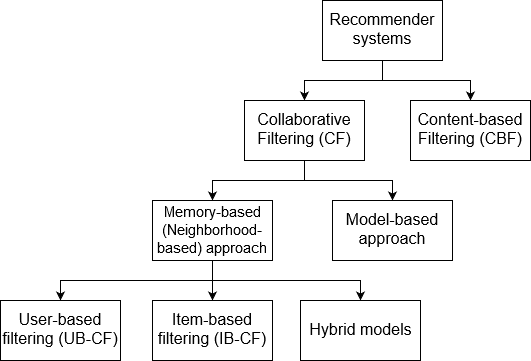
\includegraphics[scale=0.5]{images/recommender_systems.png}
	\caption{Categorizzazione generale dei sistemi di raccomandazione}
	\label{fig:recommender_systems}
\end{figure}

Entrambi gli approcci (CBF e CF) hanno i loro punti di forza e di debolezza. Il primo algoritmo si focalizza sul contenuto degli item e
sugli interessi del singolo utente e propone item differenti a utenti differenti, questo significa che ogni utente può ricevere 
raccomandazioni uniche; e questo è un vantaggio. 
Tuttavia la più grande limitazione del CBF è il fatto di non poter determinare se un utente è interessato ad un item in modo implicito,
perchè analizza solamente direttamente i metadati del prodotto e non considera gli interessi di altri utenti, i quali potrebbero 
suggerire item che non verrebero notati con questo approccio.
Per quanto riguarda il CF, nel caso siano presenti molti contenuti e proprietà associati agli item allora il sistema CF consuma molte 
risorse e tempo per poter analizzarli, nel contempo a questo algoritmo non interessano queste informazioni. Una raccomandazione 
viene fatta sulla base delle valutazioni degli utenti per gli item, o sugli usi che gli utenti fanno degli item e questo è il suo punto 
di forza perchè non si trova a dover analizzare item ricchi di informazioni. Allo stesso tempo è anche il suo punto debole, perchè può
portare a suggerimenti che potrebbero essere considerati poco adatti sulla base della poca relazione con i profili di alcuni utenti. 
Questo problema è accentuato quando sono presenti nel database molti item che non hanno valutazioni o non sono stati mai usati dagli 
utenti.
\cite{model-based-approach-for-collaborative-filtering}

Un sistema di raccomandazione filtra i dati usando differenti algoritmi e raccomanda gli item più rilevanti agli utenti, attraverso 
un procedimento a 3 fasi:

\begin{description}
	\item[Raccolta di dati]: questo è il primo step e anche quello più importante per poter costruire un sistema di 
	raccomandazione che produca risultanti rilevanti e consistenti. I dati possono essere raccolti in due modi: esplicitamente,
	cioè attraverso la raccolta diretta di informazioni fornite dagli utenti, ad esempio le valutazioni di un prodotto; mentre 
	attarverso l'approccio implicito, vengono raccolti dati che non sono prodotti in modo intenzionale dall'utente ma ottenuti
	dai costanti flussi di dati come la cronologia di ricerca, i click effettuati, lo storico degli ordini, etc.
	\item[Memorizzazione di dati]: la quantità di dati definisce quanto efficace un modello di raccomandazione possa di
	diventare. Ad esempio, in un sistema di raccomanzione per film, maggiori sono le valutazioni fornite dagli utenti, e 
	migliore sarà il sistema di raccomandazione per gli altri utenti. Il tipo di dati che si vuole raccogliere determina
	anche il supporto di memorizzazione più adatto.   
	\item[Filtraggio dei dati]: dopo la fase di raccolta e memorizzazione dei dati, essi vanno filtrati per poter estrarre
	le informazioni rilevanti per poter effettuare le raccomandazioni finali, e sono già disponibili diversi algoritmi che
	semplificano quest'ultima fase. 
\end{description}

I sistemi di raccomandazione possono essere suddivisi nelle seguenti categorie, ma speso si preferisco degli approcci imbridi cioè delle
combinazioni di sistemi di raccomandazione basati sul contenuto (\textit{Content-based filtering}) e 
quelli collaborativi (\textit{Collaborative filtering}) in modo da essere più efficaci sfruttando i pregi di entrambi gli approcci.


\subsection{Content-based filtering}
Un Content-based filtering è un sistema di raccomandazione in cui vengono suggeriti item simili a un particolare item (oggetti 
o prodotti). 

Questo approccio sfrutta i metadati dell'item, che possono essere il genere, una descrizione, uno o più autori, la categoria di 
appartenenza etc. per fare queste raccomandazioni; l'idea base che sta dietro questi raccomandatori, è che se ad un utente piace 
o interessa un particolare item allora gli piaceranno anche altri item simili.

Questo algoritmo suggerisce prodotti che piacevano all'utente nel passato ed è limitato a item dello stesso tipo. Un 
content-based recommender fa riferimento a quegli approcci, che provvedono raccomandazioni comparano la rappresentazione del
contenuto che descrive un item e la rappresentazione del contenuto dell'item interessato dall'utente. 

Questi metodi sono usati quando si sanno a priori delle informazioni sugli item che si vuole suggerire, ma non sugli utenti.
In questo sistema, delle keyword (parole chiave) sono utilizzate per caratterizzare gli item e un profilo dell'utente è 
costruito per indicare quali item gli piacciono. In altre parole, questi algoritmi cercano di raccomandare item che 
all'utente sono piaciuti o ha usato nel passato e sta esaminando nel presente. La costruzione del profilo dell'utente,
spesso temporaneo, non viene basata su un modulo di registrazione che l'utente stesso deve compilare, ma su informazioni
lasciate indirettamente dall'utente. Più precisamente, tra vari item candidati da raccomandare all'utente si passa per un 
processo di confronto con gli item piaciuti dall'utente e gli item migliori vengono suggeriti.


\subsection{Collaborative filtering}
I filtri collaborativi (\textit{Collaborative filtering}) lavorano costruendo un database di preferenze di utenti su item (o prodotti),
sfruttano tecniche di analisi dei dati al problema di aiutare gli utenti a trovare gli item che gli potrebbero piacere producendo una 
lista dei top-N item da raccomandare per un dato utente.
Un nuovo utente subisce un processo di matching all'interno del database per scoprire quali sono i possibili vicini (\textit{neighbors}),
che corrispondo agli altri utenti aventi storicamente simili preferenze al nuovo utente. Agli item maggiormente preferiti dai vicini sono
raccomandati al nuovo utente, visto che potrebbero essere di suo interesse. 

Questi sistemi tentano di predirre la valutazione o la preferenza che un utente darebbe a un item basandosi su preferenze date da altri 
utenti, queste preferenze possono essere ottenute o in modo esplicito dagli utenti o tramite qualche misurazione implicita. 
I filtri collaborativi non richiedono l'uso di metadati associati agli item come nella loro controparte, i filtri content-based. A un 
utente vengono raccomandati item basandosi su valutazioni passate collezionate da altri utenti.

Tuttavia, restano ancora oggi alcune sfide significative a cui sono sottoposti i sistemi di raccomandazione basati su 
filtraggio collaborativo.
Il primo obbiettivo è quello di migliorare la scalabilità degli algoritmi di filtri collaborativi; questi algoritmi sono in grado di cercare
anche diecimila di potenziali vicini (utenti simili) in tempo reale, ma la richiesta dei sistemi moderni è di cercare dieci milioni di 
potenziali vicini. Algoritmi esistenti hanno problemi di performance con i singoli utenti quando essi hanno molte informazioni.
Il secondo obbiettivo è quello di migliorare la qualità dei sistemi di raccomandazione per gli utenti. Gli utenti vogliono
raccomandazioni di cui possono fidarsi e che possono aiutarli a trovare item che potrebbero essere di loro gusto.
Per certi versi questi due obbiettivi sono in conflitto tra di loro e per ottenere dei risultati validi e di una certa importanza è 
necessario trattarli in contemporanea perchè aumentare solamente la scalabilità diminuirebbe la sua qualità e viceversa. 
\cite{item-based-collaborative-filtering} 

Il principale modello di filtro collaborativo studiato in questo elaborato è il metodo definito come \textit{Memory-based} e il 
vantaggio di utilizzare queste tecniche sta nel fatto di essere semplici da implementare e i risultati ottenuti sono altrettanto 
semplici da spiegare; mentre ci possono essere anche filtri collaborativi che sfruttano metodi \textit{Model-based} che si basano sulla 
fattorizzazione di matrici e sono molto più funzionali per gestire il problema della sparsità dei dati. Questi ultimi sono sviluppati
usando algoritmi di data mining e machine learning per predirre le valutazioni di utenti su item senza valutazioni, inoltre sono spesso 
associati a tecniche come la dimensionality reduction per migliorare la precisione.


\paragraph{Model-based filtering} 
Gli algoritmi Model-based tentano di comprimere grandi database in un modello ed effettuare il processo di raccomandazione applicando dei
meccanismi di riferimento all'interno di questo modello. 
I CF Model-based posssono rispondere alle richieste degli utenti istantaneamente. \cite{model-based-approach-for-collaborative-filtering}


\subsection{Cold Start problem} 
Cosa succederebbe se un nuovo utente o un nuovo item è aggiunto al dataset? Questa situazione è chiamata \textit{Cold Start}. Ci possono
essere due tipi di Cold Start:
\begin{description}
	\item[Visitor Cold Start]: si verifica quando un nuovo utente è stato aggiunto al database, visto che non c'è alcuno storico relativo ad esso, il sistema non
	sa le le sue preferenze; per questo motivo diventa molto più difficile raccomandare prodotti a quel particolare utente. Per risolvere questo problema,
	a livello teorico, si potrebbe applicare un procedimento di raccomandazione basata sulla popolarità dei prodotti, ma solo una volta che si è venuti a 
	conoscenza delle preferenze dell'utente, sarà possibile generare delle raccomandazioni più precise e adeguate alle sue esigenze.
	\item[Item Cold Start]: si verifica quando un nuovo item viene inserito nel sistema. L'azione dell'utente è quella più importante per determinare
	il valore di questo item; maggiore l'interazione un item riceve, più è facile che venga raccomandato all'utente giusto.  
\end{description}



